To explore these relationships, we used the Million Song Dataset.
This is a freely-available dataset consists of features and metadata on one million contemporary songs,
produced by The Echo Nest.
While the dataset does not include actual audio,
its features include a large variety of measurements.

Many features come from analyzing segments of a song:
each song is divided into many segments, and measurements are made on each segment.
These measurements include features such as loudness or pitch.
Other features are more summary variables on the entire song, such as "danceability."
For the purposes of our analysis, we focused on the segmented features,
and did not use any "summary" variables.
We did this to see if we could identify aural commonalities within the songs themselves,
rather than broad measurements of the entire song.

\begin{figure*}[ht]
    \centering
    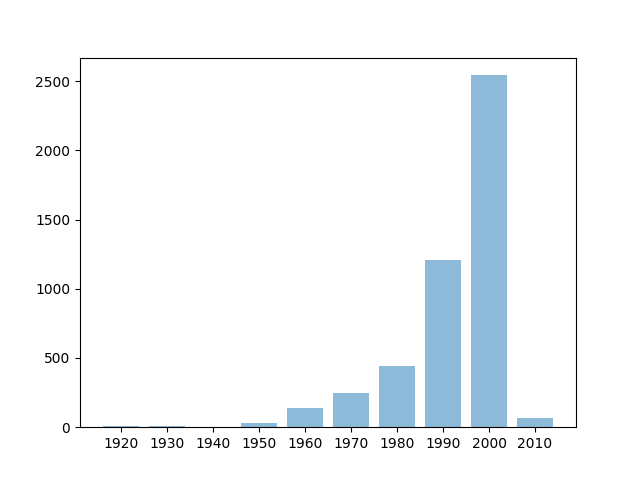
\includegraphics[width=.9\textwidth]{decade_counts}
    \caption{Data Distribution across Decades}
    \label{fig:decade}
\end{figure*}

We preprocessed these segmented measures by using the idea of k-grams.
That is, for a measure like "loudness", we took $k$ consecutive measures of loudness
in a song, and 
count that particular sequence of loudness as a unique variable.
We then represent each song as a count of the occurrences of each sequence for every variable.
Thus our preprocessed dataset is a sparse matrix of counts for each unique variable.

It should be noted that while our dataset is titled the Million Song Dataset,
much of this data is no longer available through the means listed at the project website.
Thus we ran our experiments on a 1\% subset of the data (totalling 10,000 songs).
While this is unfortunate, we feel that our conclusions in this report likely apply to
the larger dataset as well.
